At a hadron collider, the most fundamental tests of electroweak boson couplings
to fermions are measurements of the kinematic properties of Drell-Yan (DY)
lepton pair production.  At leading order, Drell-Yan production occurs when a
quark--anti-quark pair in the intial state annihilates into an electroweak
boson, which subsequently decays to a lepton pair. Differential cross section
calculations exist for next-to-next-to leading order (NNLO) QCD corrections as
well as NLO electroweak corrections. In the EFT context, such a
process is sensitive to four-fermion contact interactions of the type

\begin{equation}\label{lagrangian}
\begin{array}{r@{\,}c@{}c@{\,}l@{\,}l}
\mathcal L = \frac{g^2}{\Lambda^2}\;[ && \eta_{\rm LL}&\, (\overline q_{\rm L}\gamma_{\mu} q_{\rm L})\,(\overline\ell_{\rm L}\gamma^{\mu}\ell_{\rm L}) \nonumber \\
& +&\eta_{\rm RR}& (\overline q_{\rm R}\gamma_{\mu} q_{\rm R}) \,(\overline\ell_{\rm R}\gamma^{\mu}\ell_{\rm R}) \\
&+&\eta_{\rm LR}& (\overline q_{\rm L}\gamma_{\mu} q_{\rm L}) \,(\overline\ell_{\rm R}\gamma^{\mu}\ell_{\rm R}) \\
&+&\eta_{\rm RL}& (\overline q_{\rm R}\gamma_{\mu} q_{\rm R}) \,(\overline\ell_{\rm L}\gamma^{\mu}\ell_{\rm L})& ] \: ,\nonumber
\end{array}
\end{equation}
where $g$ is a coupling constant, $\Lambda$ is the contact interaction scale,
and $q_{\rm L,R}$ and $\ell_{\rm L,R}$ are left-handed and right-handed quark and
lepton fields, respectively. The parameters $\eta_{i,j}$ denote the relative interference of the operators;
the experiments have considered the cases $\eta_{\rm LR} = \eta_{\rm RL} = \pm 1$,
$\eta_{\rm LL} = \pm 1$, or $\eta_{\rm RR} = \pm 1$.

Experiments select electron or muon pairs above trigger thresholds: CMS selects
leading lepton $\pt >$ 17 GeV and second leading lepton $\pt >$ 8 GeV inclusively,
and ATLAS selects high mass events with both lepton $\pt >$ 25 GeV.  Backgrounds to Drell-Yan production
are relatively small, and consist of real prompt lepton pair production from top quark or boson pairs,
as well as fake electrons from QCD jets.  The real lepton pair background is flavor democratic,
and can therefore be reliably estimated from $e\mu$ pair production.  Fake electron production
is typically estimated from background enriched QCD jet samples, from which the fake electron rate can be measured,
convolved with electron-jet control samples.

Figure~\ref{fig:ss-inclboson-drellyan-atlas7tev} shows the Drell-Yan cross
section at high electron pair mass measured by ATLAS at 7 TeV~\cite{Aad:2013iua}.
The cross section uncertainty is predominantly systematic below 400 GeV in pair
mass and predominantly statistical above 400 GeV.  The data are compared with an NNLO QCD
prediction with NLO electroweak corrections, provided by the \texttt{FEWZ} 3.1 generator~\cite{Melnikov:2006kv,Gavin:2010az,Li:2012wna}.
The prediction also includes photon induced lepton pair production, which generally
increases cross section estimates by a few percent. The FEWZ prediction generally underestimates the cross section,
however a correlated chi-squared analysis concludes that this is not statistically significant.

Figure~\ref{fig:ss-inclboson-drellyan-cms8tev} shows the Drell-Yan cross section for electron or muon pairs
measured by CMS at 8 TeV~\cite{CMS:2014jea}.  Agreement with the FEWZ prediction is observed over the
entire measured mass range, from 15 GeV to 2000 GeV.  CMS has also measured the double differential
cross section with respect to dilepton rapidity in several bins of dilepton mass, as well as a differential
cross section ratio between the 8 TeV and 7 TeV data, which has small experimental and theoretical uncertainties.

In the absence of observed disagreements with predictions at the highest dilepton masses, the data are analyzed
to constrain the size of anomalous contact interactions. Assuming a fixed, strong value for the coupling ($g^2/4\pi = 1$),
limits can be obtained on the contact interaction scale $\Lambda$.  ATLAS estimates a lower limit of 17 to 26 TeV on $\Lambda$, where the
strongest lower limits correspond to constructive interference scenarios (especially LR+RL), and the weakest to destructive interference scenarios~\cite{Aad:2014wca}.
CMS has limits with similar sensitivity estimated for LL contact interactions~\cite{Khachatryan:2014fba}.

%ATLAS low-mass Drell-Yan $7 \TeV$~\cite{Aad:2014qja}
%ATLAS Z PT $7 \TeV$~\cite{Aad:2014xaa}
%ATLAS Z phistar $7 \TeV$~\cite{Aad:2012wfa}
%CMS Drell--Yan $7 \TeV$~\cite{Chatrchyan:2013tia}
%CMS angular coefficients $8 \TeV$~\cite{Khachatryan:2015paa}
%CMS Z PT and rapidity $8 \TeV$~\cite{Khachatryan:2015oaa}
%CMS dilepton contact interactions~\cite{Khachatryan:2014fba}
%ATLAS dilepton contact interactions~\cite{Aad:2014wca}

\begin{figure}[p]
    \centering
    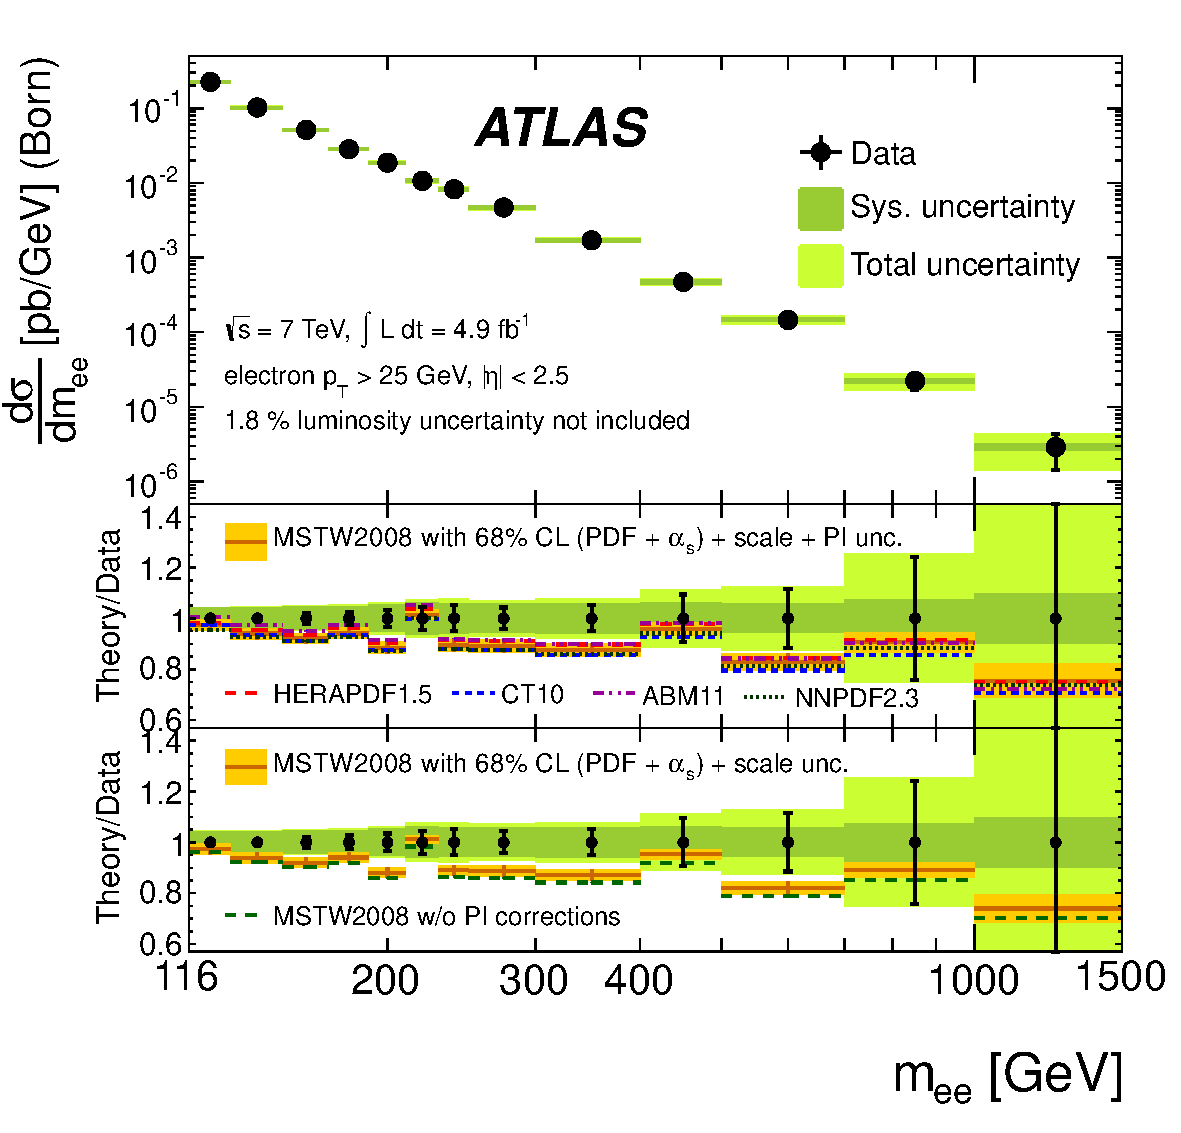
\includegraphics[height=0.3\textheight]{figures/ss-inclboson-drellyan-atlas7tev}
    \caption{Measured differential cross-section at the Born level within the
    fiducial region (electron $\pt > 25 \GeV$ and $|\eta| < 2.5$) with statistical,
     systematic, and combined statistical and systematic (total) uncertainties,
     excluding the 1.8\% uncertainty on the luminosity.
      On the left, in the upper ratio plot, the photon-induced (PI)
     corrections have been added to the predictions obtained from the MSTW2008,
     HERAPDF1.5, CT10, ABM11 and NNPDF2.3 NNLO PDFs, and for the MSTW2008 prediction
     the total uncertainty band arising from the PDF, $\alpha_s$, renormalisation
     and factorisation scale, and photon-induced uncertainties is drawn. The lower
     ratio plot shows the influence of the photon-induced corrections on the
     MSTW2008 prediction, the uncertainty band including only the PDF, $\alpha_s$
     and scale uncertainties.}
    \label{fig:ss-inclboson-drellyan-atlas7tev}
\end{figure}

\begin{figure}[p]
    \centering
    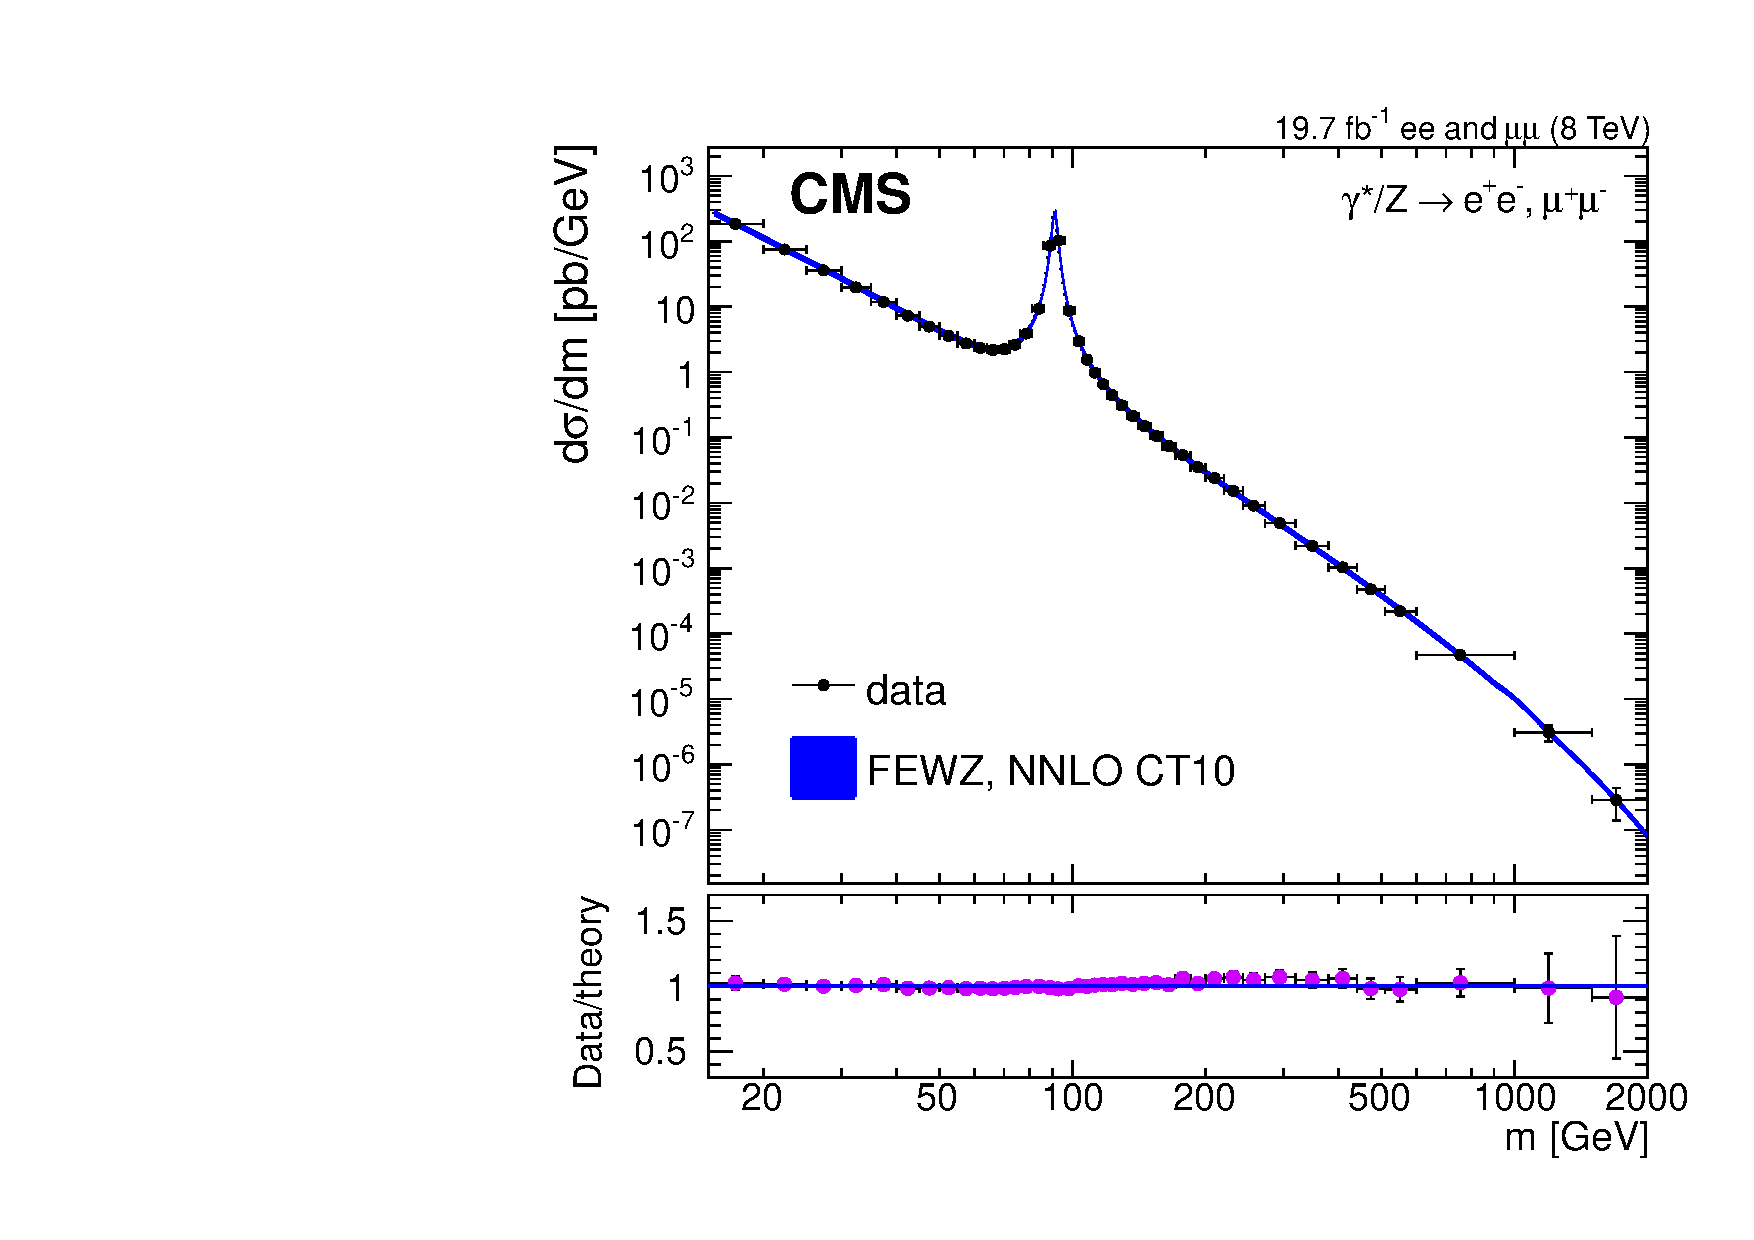
\includegraphics[height=0.3\textheight]{figures/ss-inclboson-drellyan-cms8tev}
    \caption{The DY differential cross section as measured in the combined
dilepton channel and as predicted by NNLO FEWZ 3.1 with CT10 PDF
calculations, for the full phase space.}
    \label{fig:ss-inclboson-drellyan-cms8tev}
\end{figure}
